\section{Fase 4: Análisis Exploratorio de datos oncológicos}

En esta fase, el científico obtiene el conjunto de datos o imágenes que fueron organizados previamente por el ingeniero y realiza un \textit{Análisis exploratorio de datos} para descubrir patrones generales en la información generada. Cabe resaltar, que en esta fase el acompañamiento del medico experto en oncología es de vital importancia, ya que los datos o imágenes que van ser explorados por el científico pueden contener variables que pueden tener o no un valor significativo para el experto, ayudando así a determinar si el análisis planteado para responder la pregunta va o no por un buen camino, de modo que es posible que se agreguen o eliminen diversas variables para lograr el resultado esperado. Adicionalmente, es necesario que los diversos análisis generados estén apoyados con gráficas que sean entendibles por todo el \textit{Data Analysis Team}, esto con el proposito de aportar ideas, y desde esta fase ir encontrando posibles correlaciones entre las variables oncológicas.

\subsection{Análisis Descriptivo}
En primer lugar, se realizo el respectivo análisis descriptivo para detectar cual es comportamiento de los atributos del conjunto de datos \textit{“Breast Invasive Carcinoma (TCGA, Cell 2015)”}. En la gráfica \ref{EDA_2} se puede observar las gráficas estadísticas unidimensionales de la 110 variables, las cuales permitieron extraer  las características mas representativas y permitieron identificar el comportamiento de los datos.

\begin{itemize}[label=\HandPencilLeft]
	\item El conjunto de datos esta conformado por 95 variables \textit{Categóricas} y 15 variables \textit{Numéricas}.
	
	\item Dada la naturaleza de las preguntas planteadas en el BCQM en donde se busca la identificación de características genéticas, las variables \textit{Study ID, Patient ID, Sample ID, Other Patient ID, Other Sample ID, Form completion date y Pathologyc Report File Name} no generan un aporte significativo para encontrar una respuesta de valor, dado lo anterior fueron eliminadas del conjunto de datos con el cual se entrenaron a los modelos de ML.
	
	\item 
\end{itemize}


\newpage
\begin{figure}
	\centering
	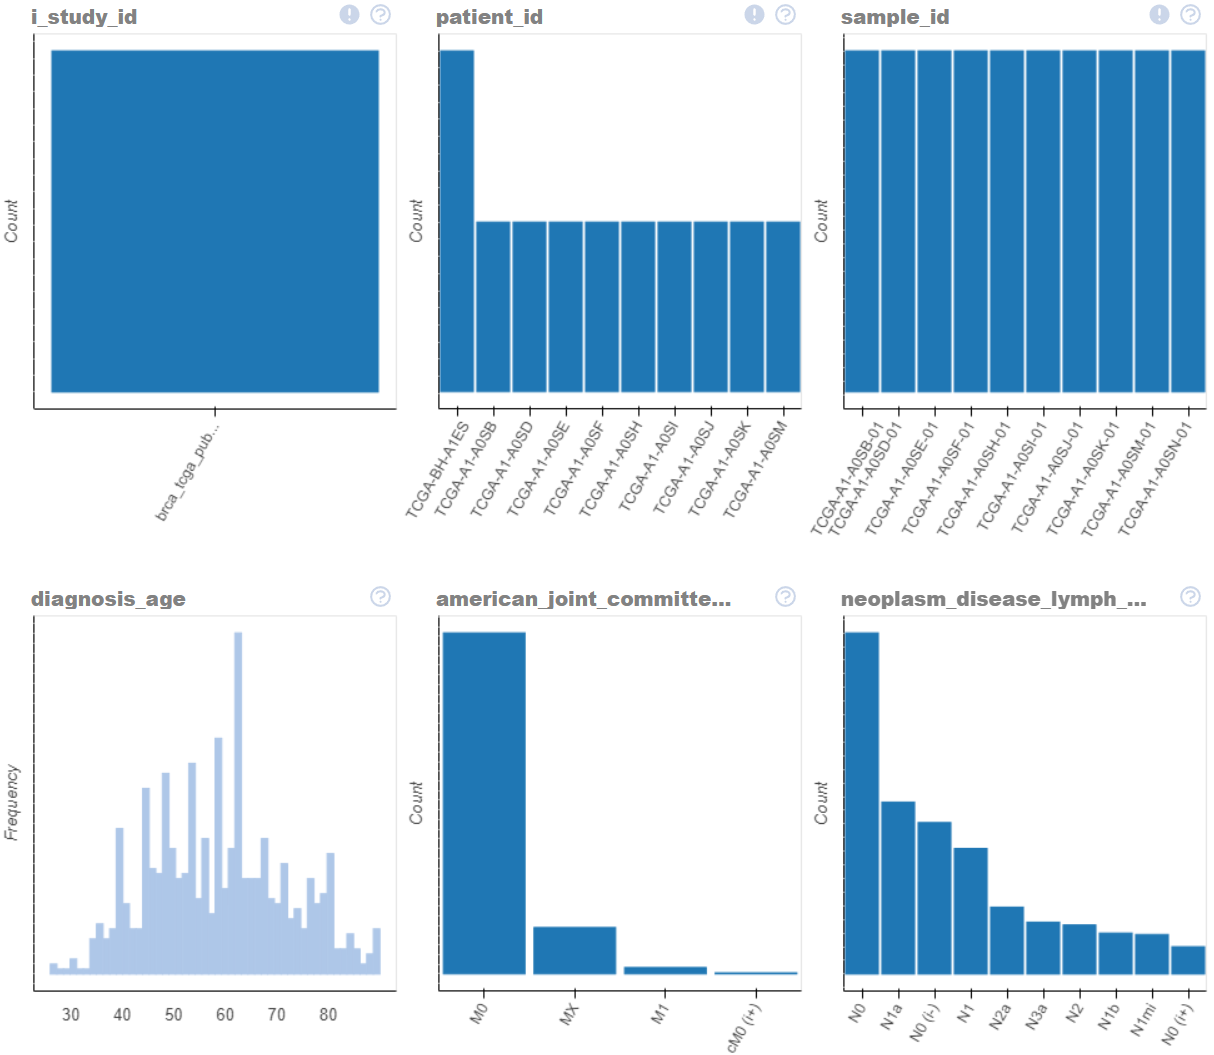
\includegraphics[width=1
	\linewidth]{NOTEBOOK/IMAGES_EDA/1}
\end{figure}

\begin{figure}
	\centering
	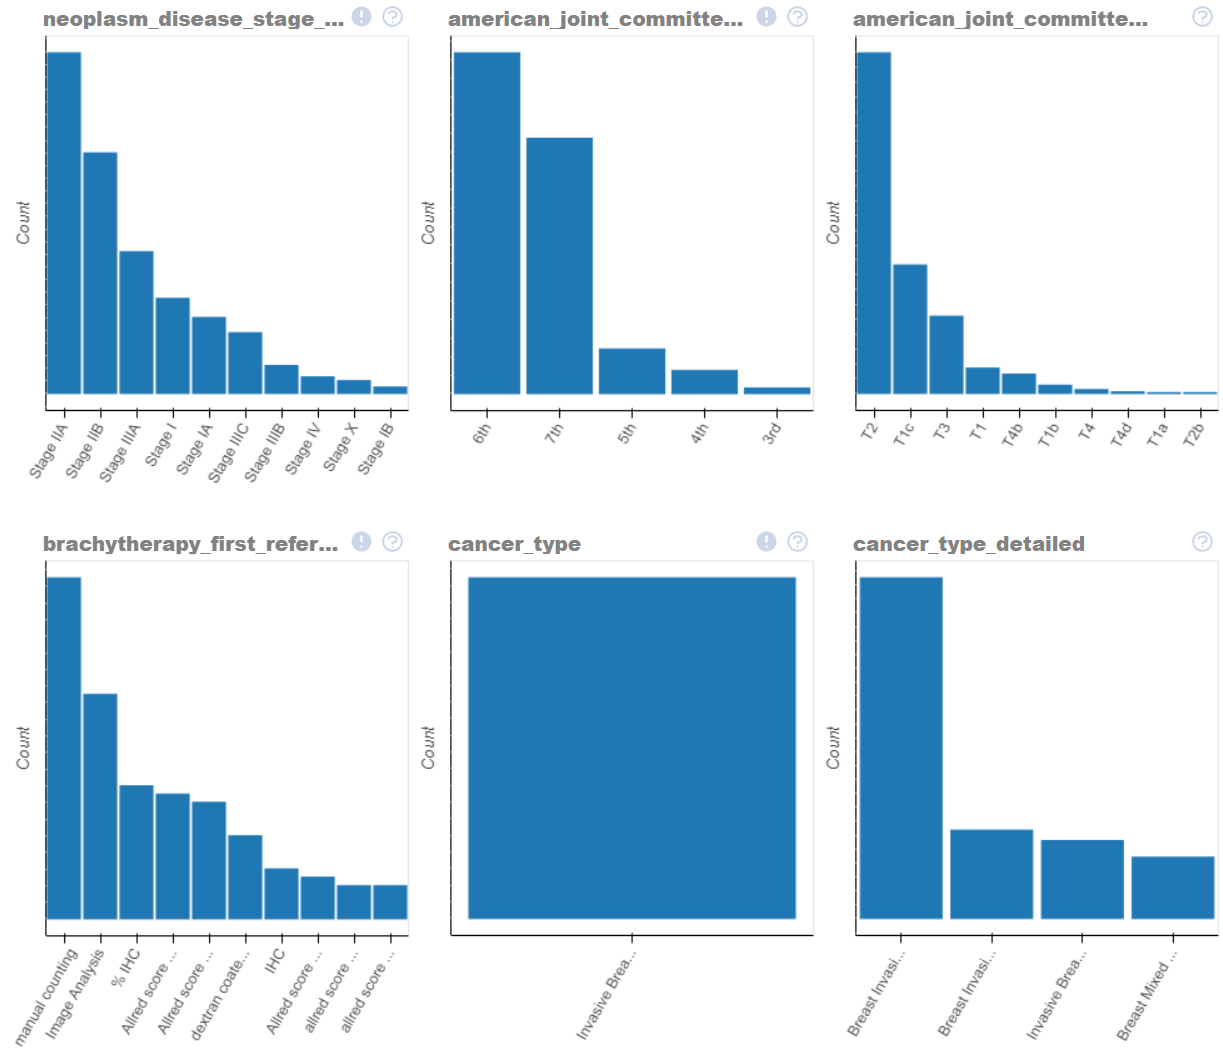
\includegraphics[width=1
	\linewidth]{NOTEBOOK/IMAGES_EDA/2}
\end{figure}

\begin{figure}
	\centering
	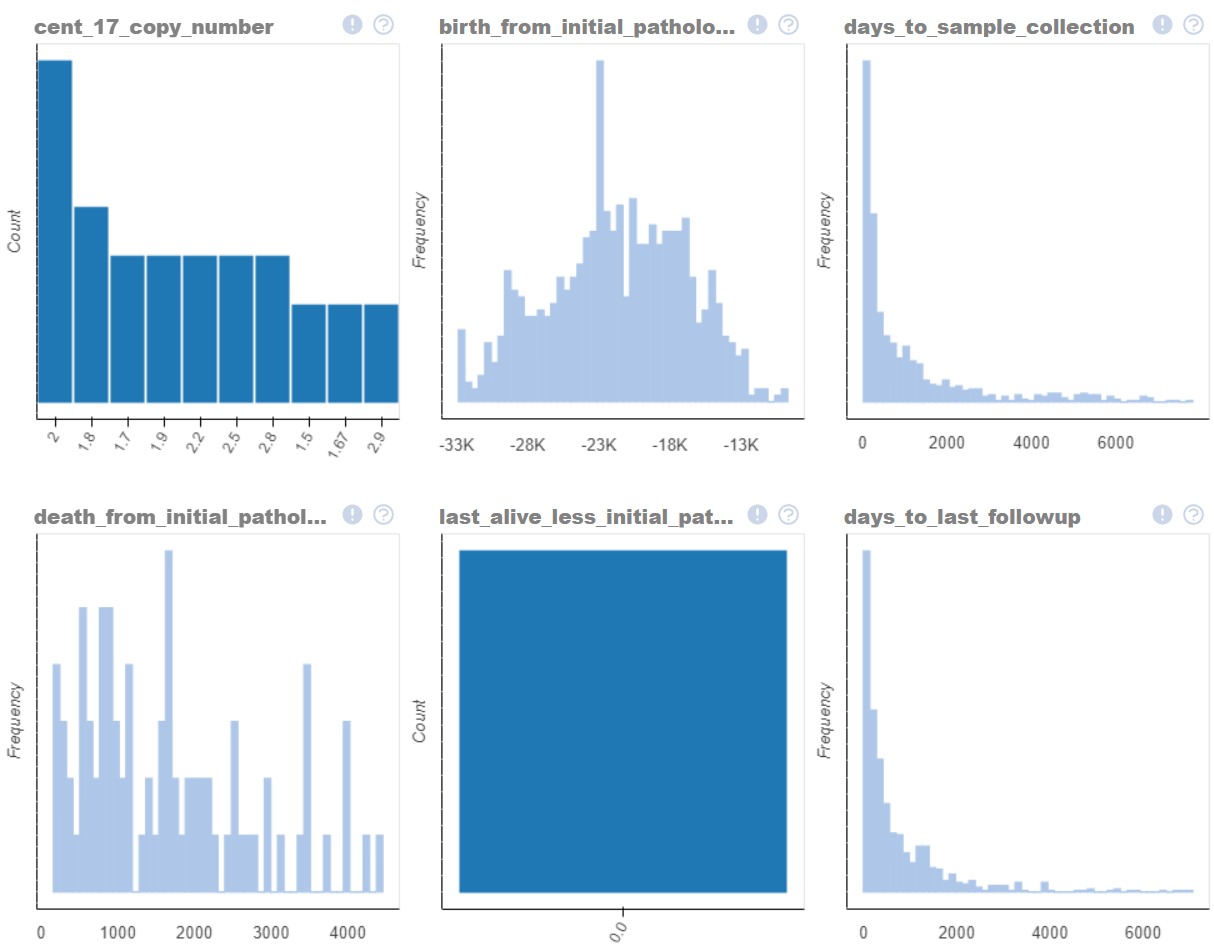
\includegraphics[width=1
	\linewidth]{NOTEBOOK/IMAGES_EDA/3}
\end{figure}

\begin{figure}
	\centering
	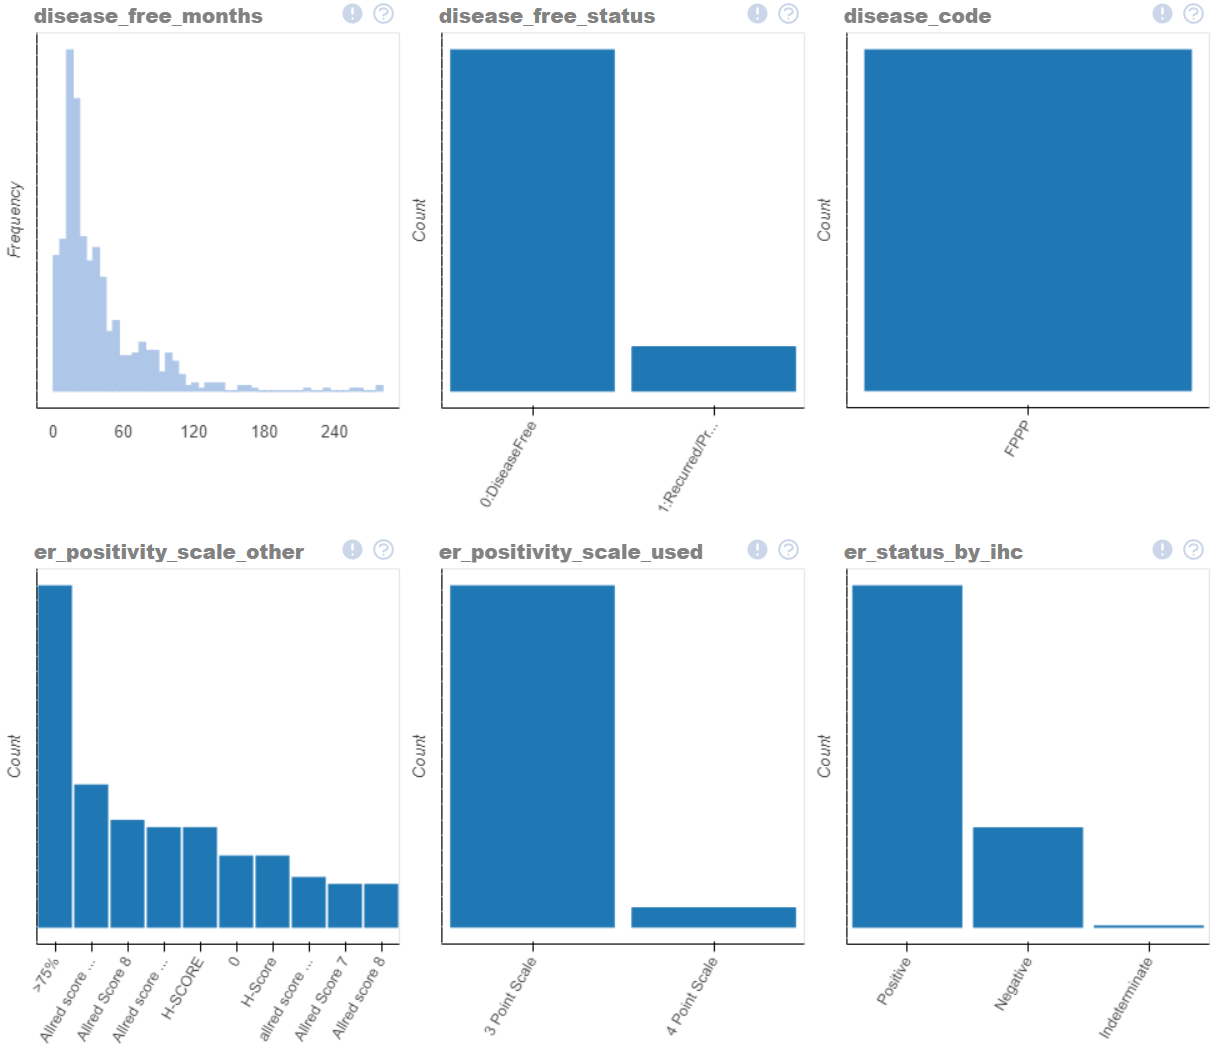
\includegraphics[width=1
	\linewidth]{NOTEBOOK/IMAGES_EDA/4}
\end{figure}

\begin{figure}
	\centering
	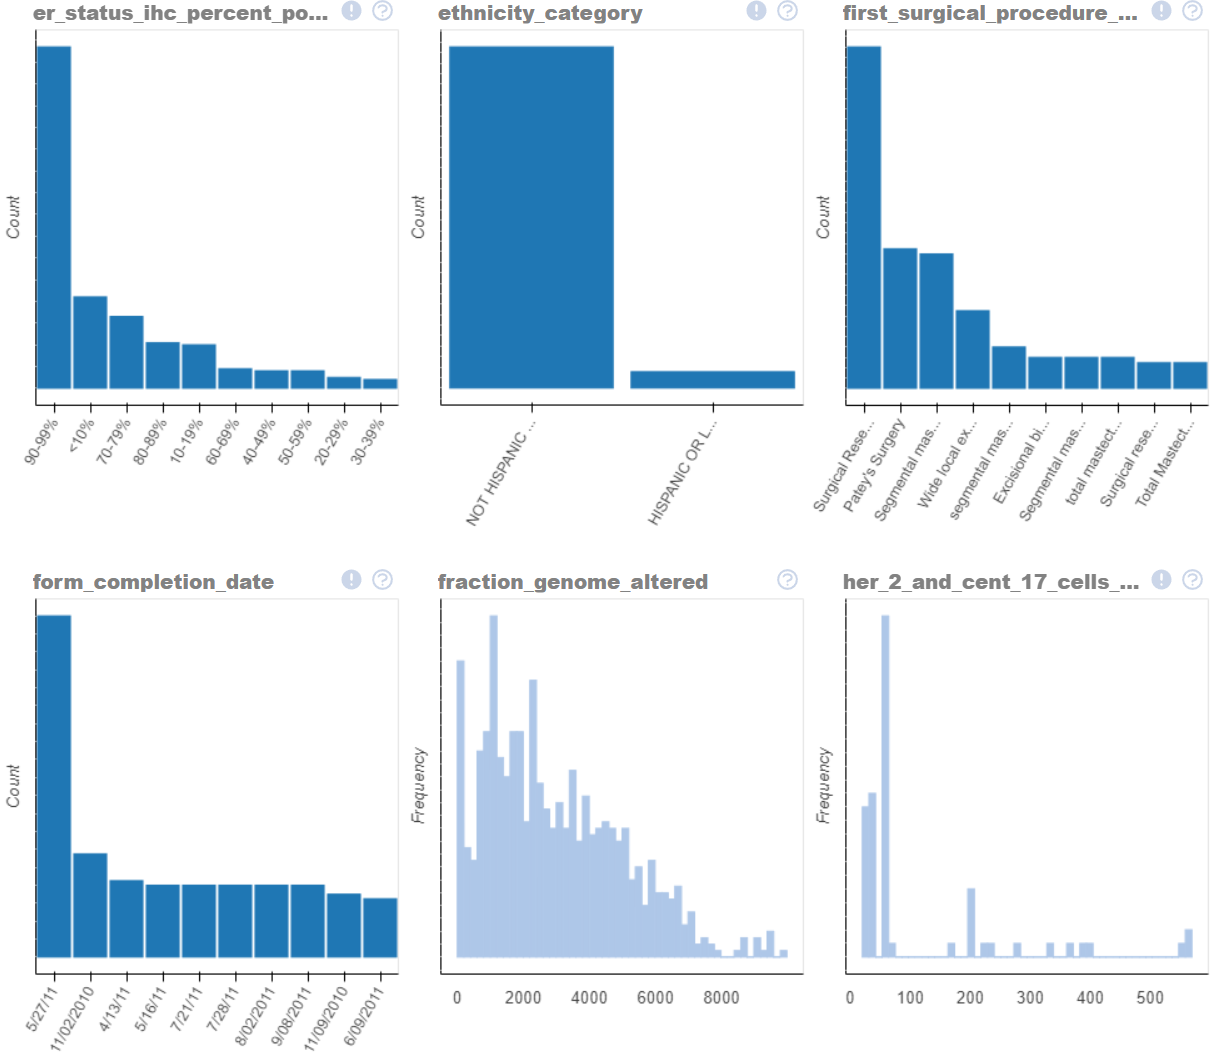
\includegraphics[width=1
	\linewidth]{NOTEBOOK/IMAGES_EDA/5}
	\caption{Distribuciones del conjunto de datos del Carcinoma invasivo de mama.}\label{fig:foobar}
\end{figure}


\subsection{Detección de datos Ausentes}
En segundo lugar, basados en la obtención de los atributos del conjunto de datos \textit{“Breast Invasive Carcinoma (TCGA, Cell 2015)”}, se realizo un análisis de la cantidad de datos perdidos para identificar las variables y en la etapa posterior realizar la limpieza y el pre-procesamiento de los datos de destino hacerlos consistentes y sin ningún tipo de ruido. Los resultados obtenidos se pueden observar en la figura \ref{Missing_Bar_Chart}:


\begin{figure}[!htb]
	\centering
	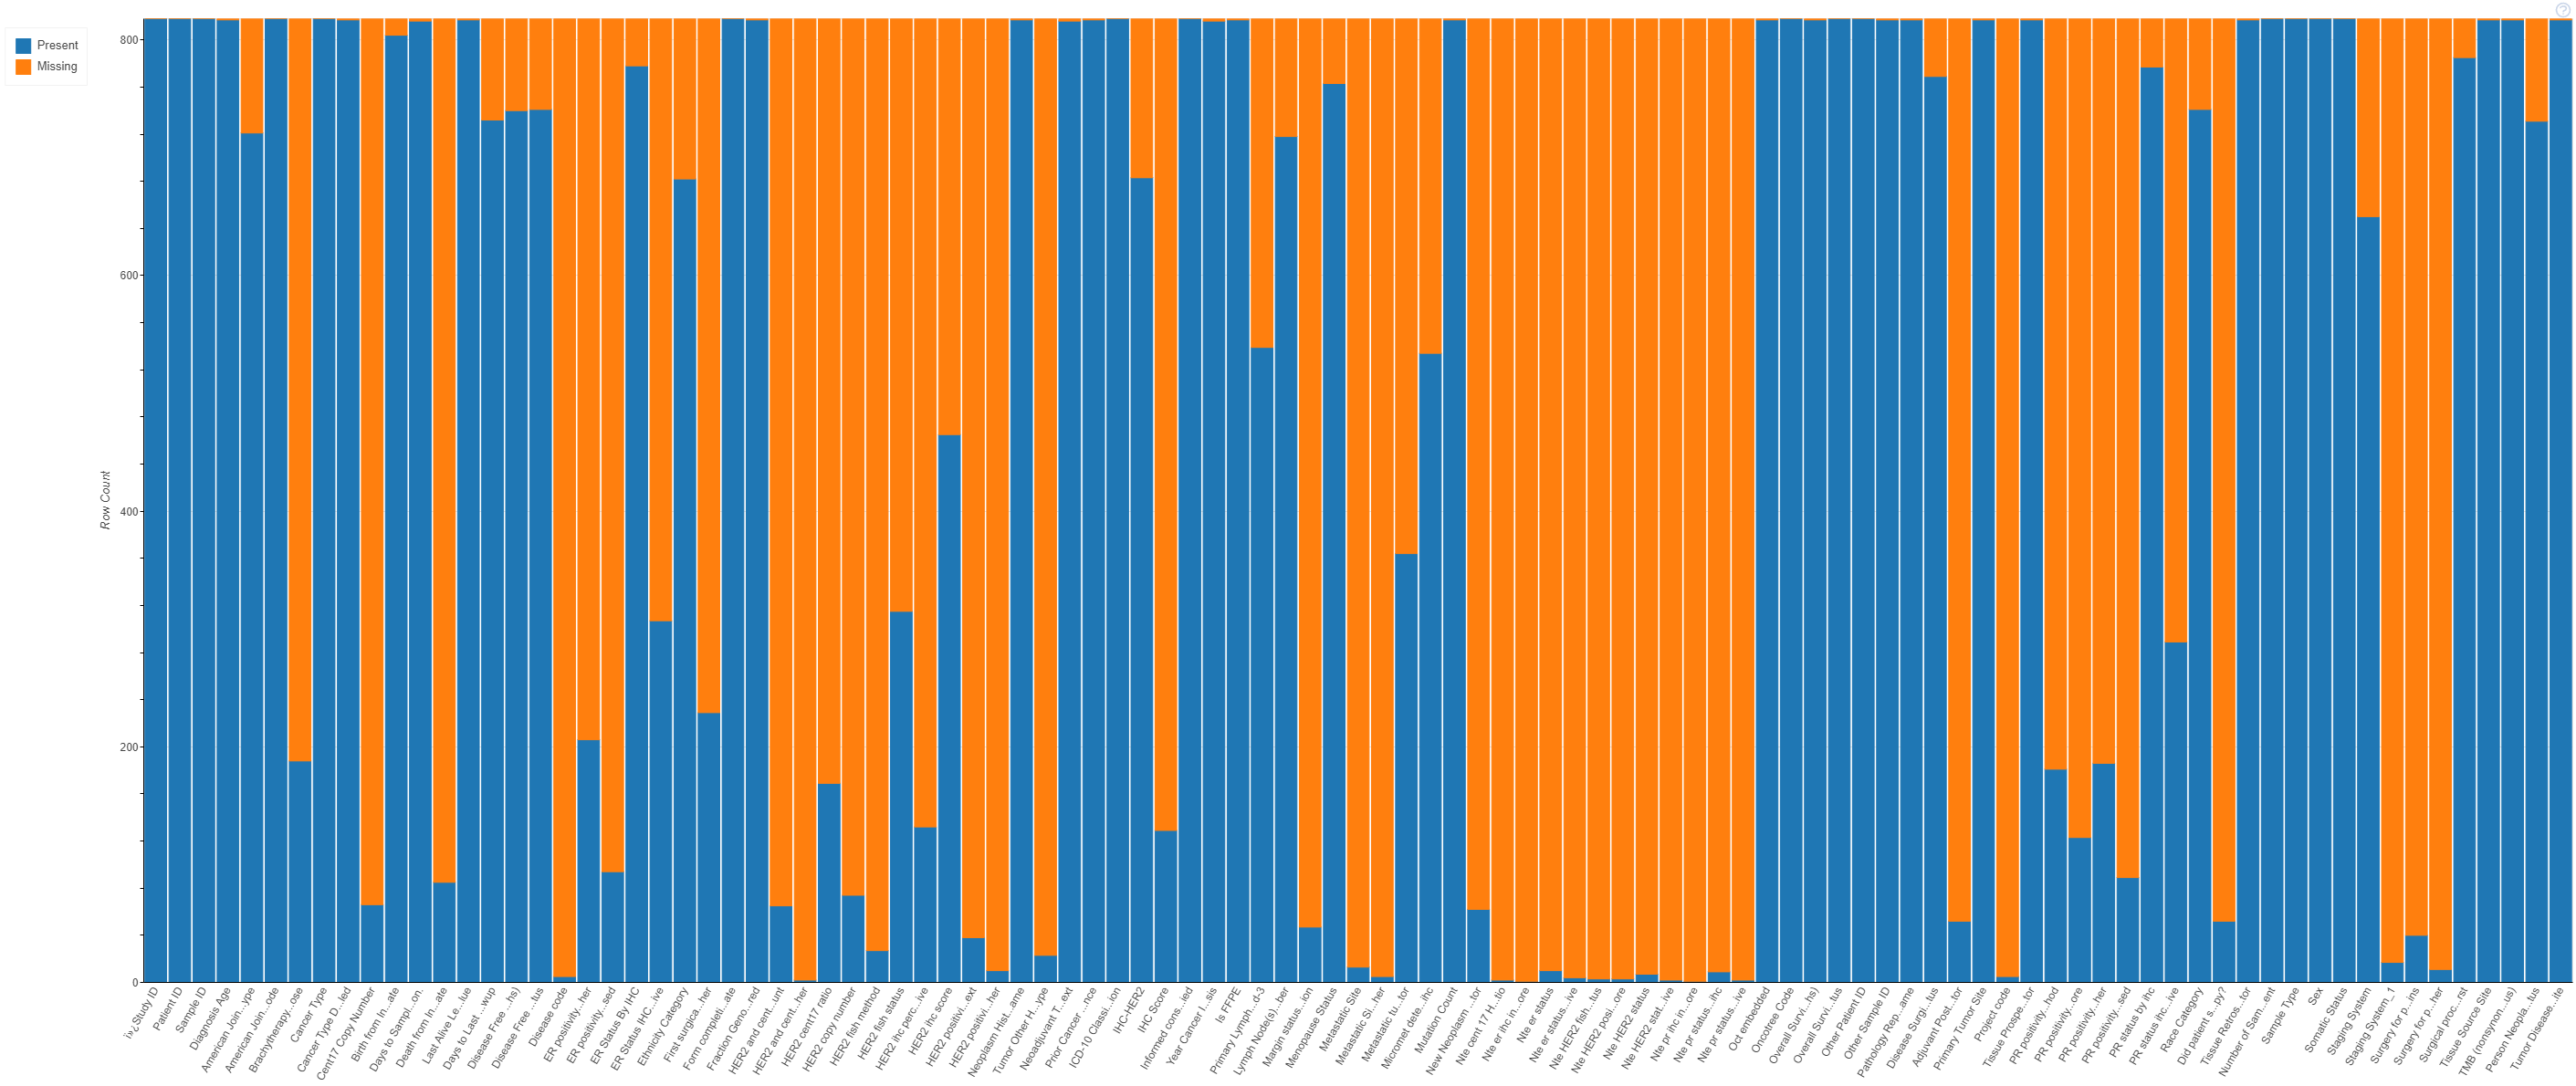
\includegraphics[width=1
	\linewidth]{IMAGENES/Missing_Bar_Chart}
	\caption{Datos perdidos expresados en una gráfica de barras.}
	\label{Missing_Bar_Chart}
\end{figure}

\begin{figure}[!htb]
	\centering
	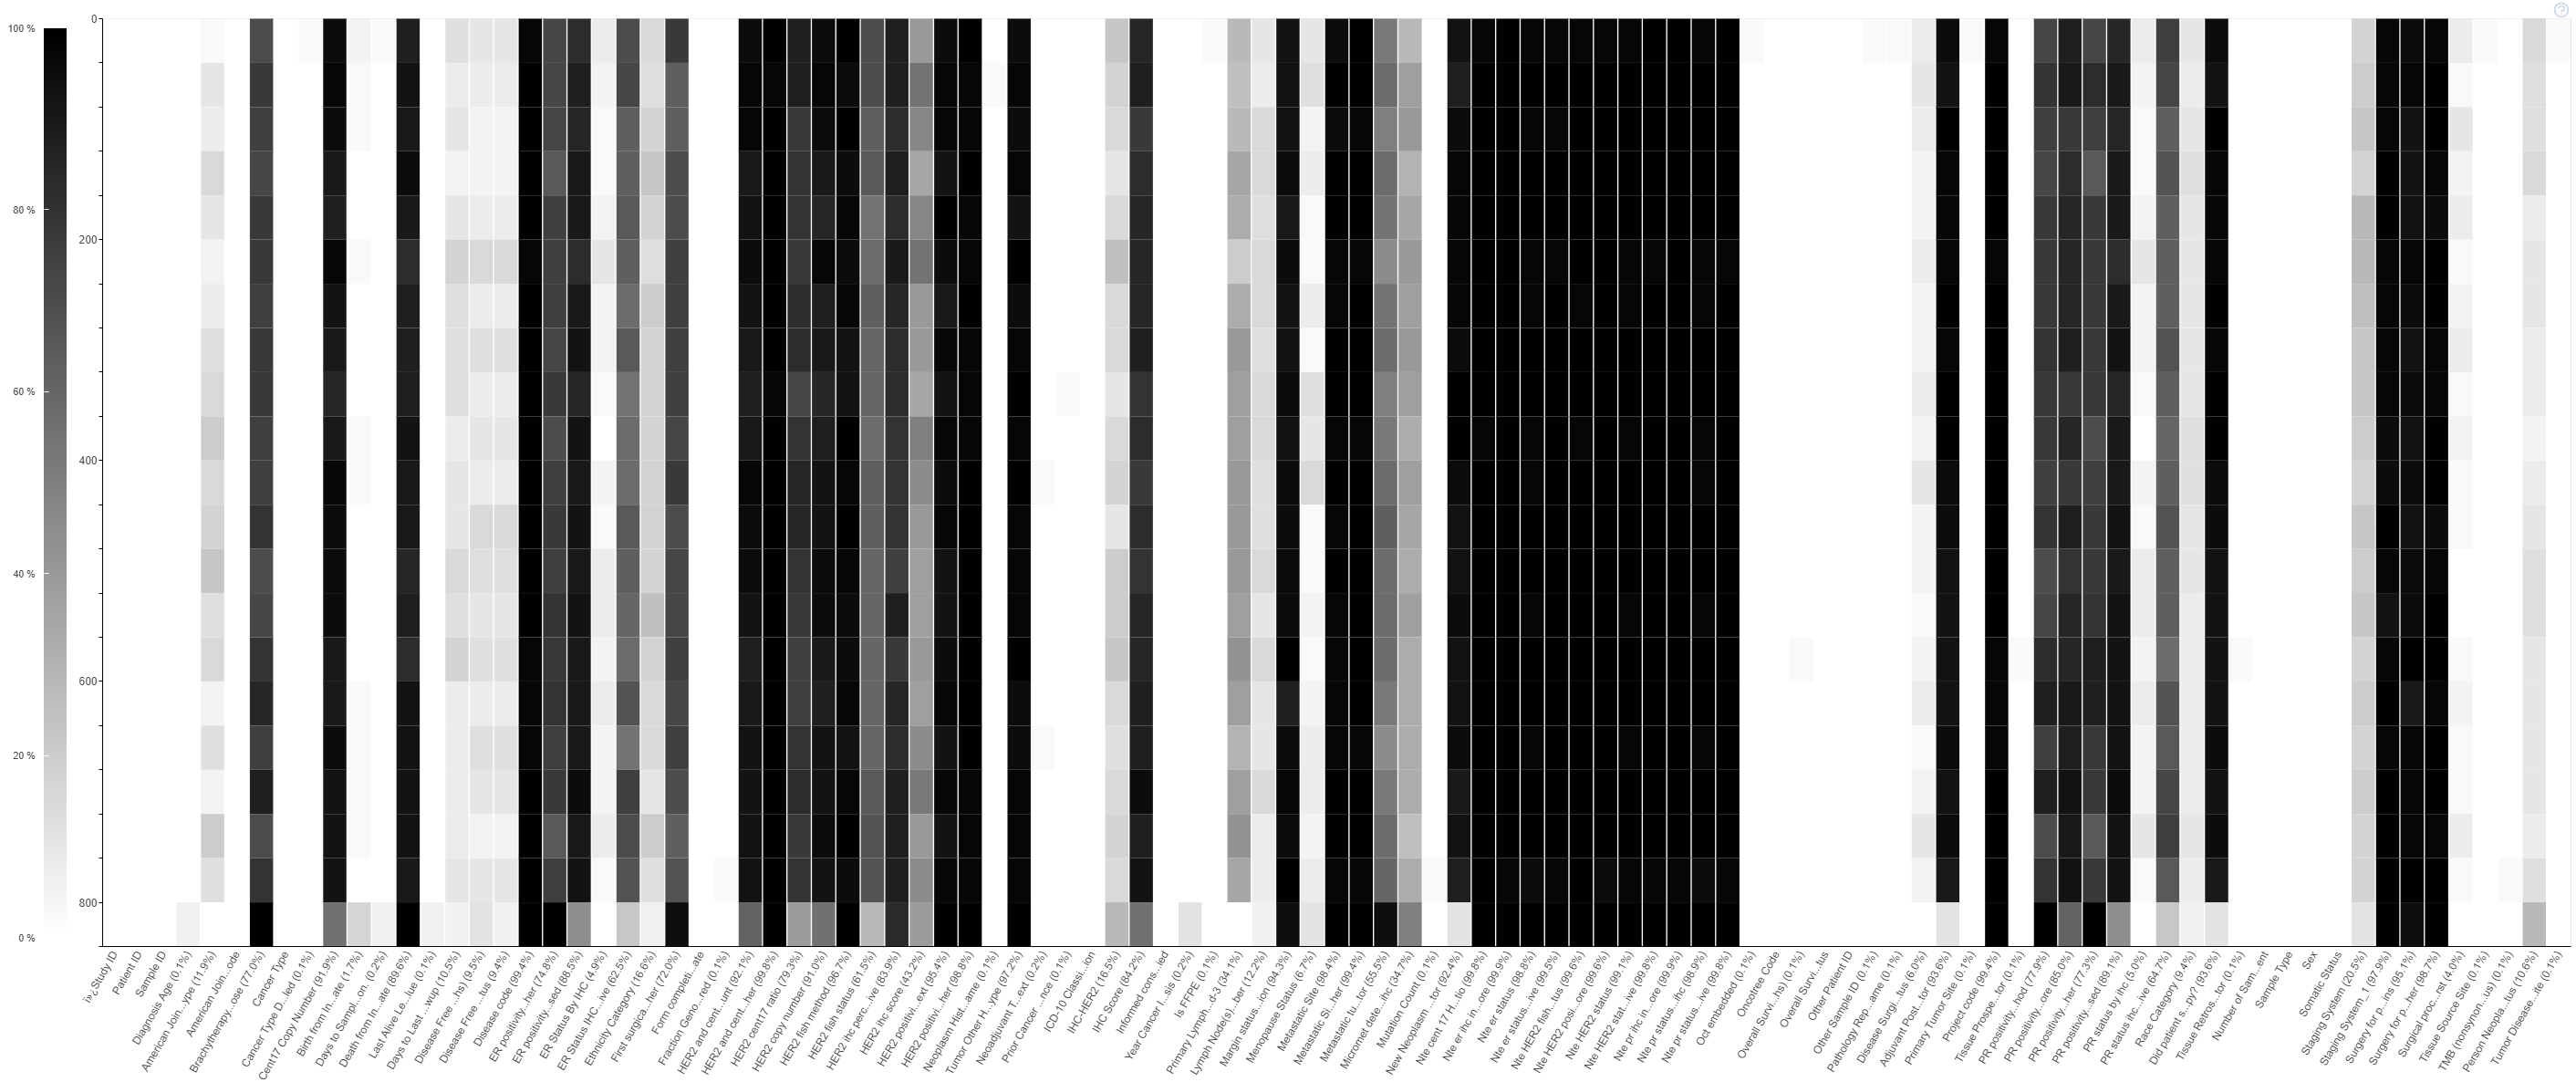
\includegraphics[width=1
	\linewidth]{IMAGENES/Missing_Spectrum}
	\caption{Datos perdidos expresados en un diagrama espectral.}
	\label{Missing_Spectrum}
\end{figure}

